\documentclass[a4paper,12pt]{article}
\usepackage[left=78bp,right=78bp,top=68bp,bottom=62bp]{geometry}
\usepackage{fontspec,graphicx}
\setmainfont{Times New Roman}
\pagestyle{empty}
\setlength\parindent{0pt}
\newcommand{\viewcaption}[1]{\par\smallskip{\fontsize{10bp}{12bp}\selectfont\itshape #1\par}}
\begin{document}
{\fontsize{15bp}{19bp}\selectfont\bfseries Appendix D. Native DIALux false-colour views\par}
\bigskip
\textbf{D.1 Room surfaces}\par\smallskip
\begin{center}
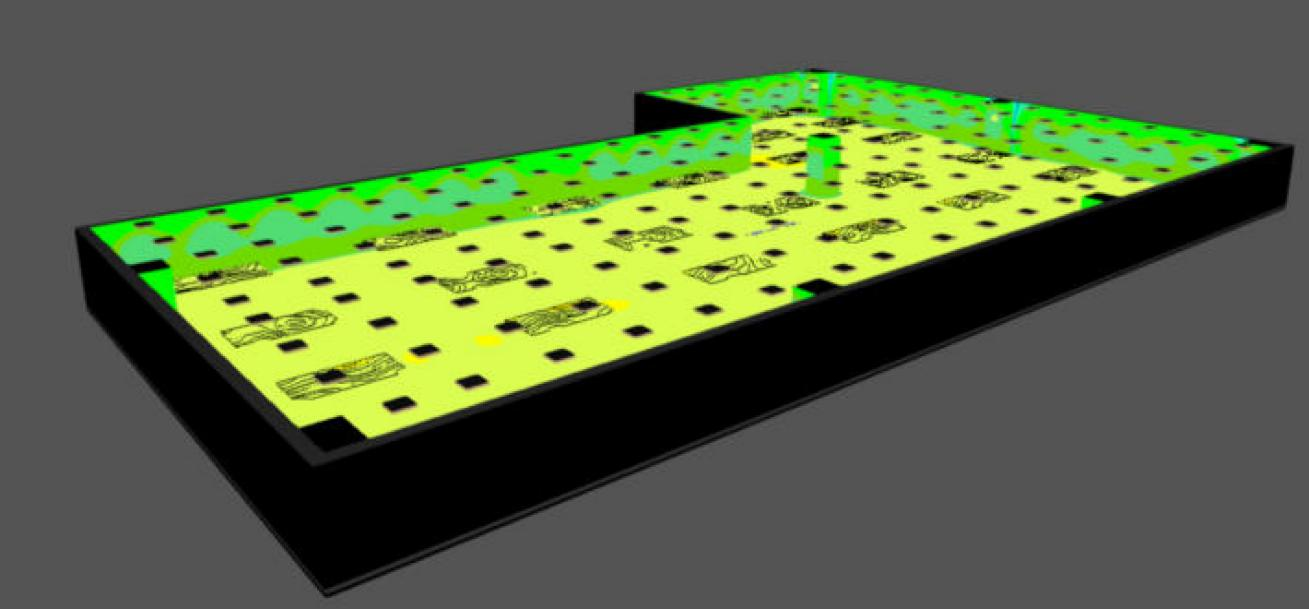
\includegraphics[width=.93\linewidth]{../Assets/room-false-colours.jpg}
\viewcaption{Figure D1. Baseline room surfaces in false colour, with isolux contours on the desk calculation surfaces.}
\end{center}
\medskip
\textbf{D.2 Desk calculation surfaces}\par\smallskip
\begin{center}
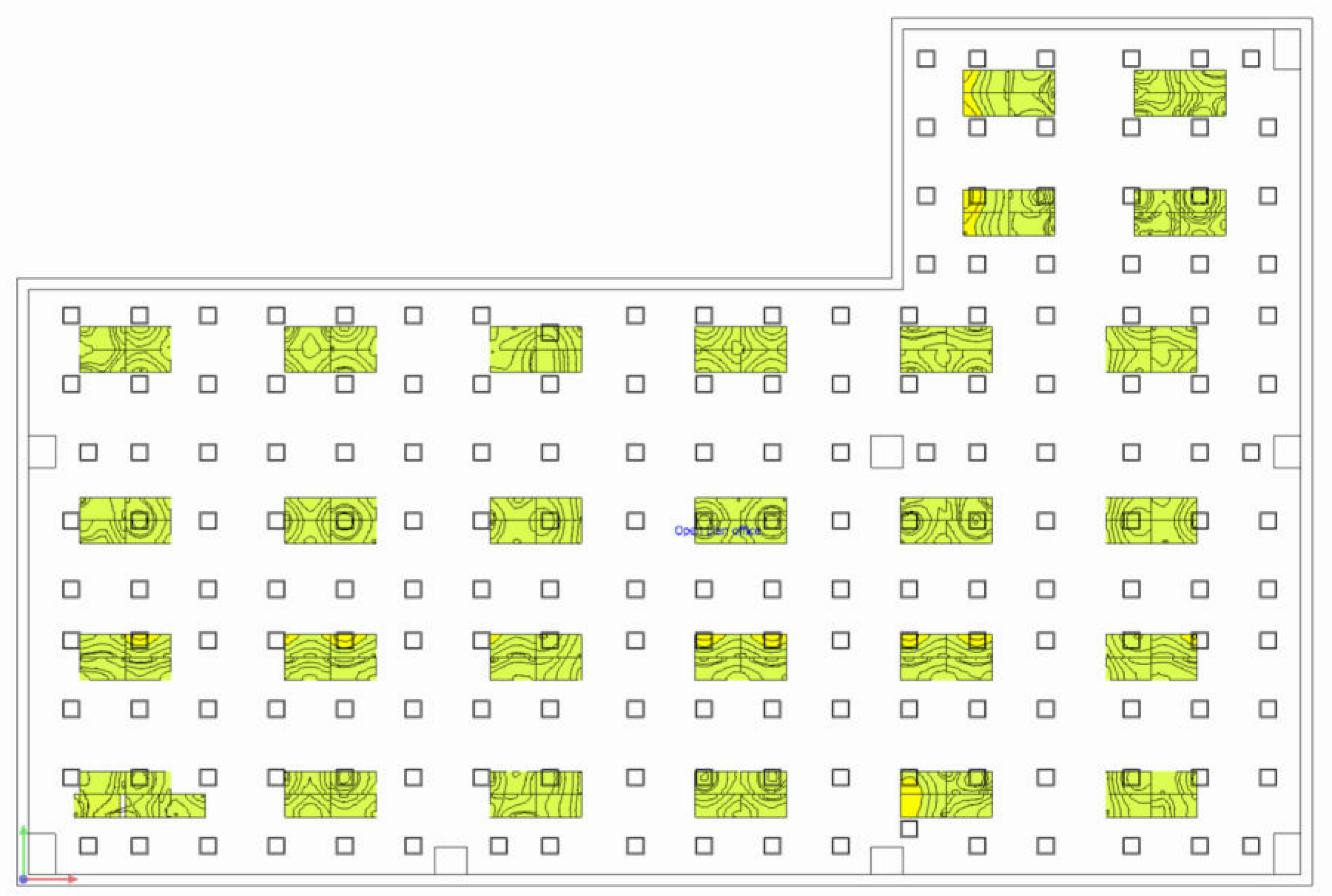
\includegraphics[width=.78\linewidth]{../Assets/desk-false-colours.jpg}\\[2bp]
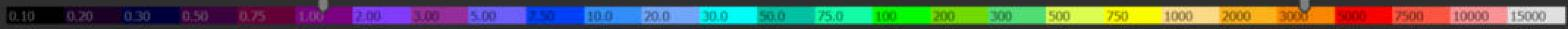
\includegraphics[width=\linewidth]{../Assets/illuminance-scale.jpg}
\viewcaption{Figure D2. False colours show local illuminance at 0.8 m (scale in lx). Across the 112 desks, maintained desk means range from 593 to 742 lx. Individual grid points range from 513 to 814 lx.}
\end{center}
\end{document}
